\newpage
\section*{Metasivu}


Kirjan julkaisee avoimeen levitykseen Metropolia AMK:n Vesa Linja-ahon koordinoima Oppikirjamaraton-projekti yhteistyössä Avoimet oppimateriaalit ry:n kanssa Teknologiateollisuuden 100-vuotissäätiön tuella.

Kirjan LaTeX-lähdekoodi: \\
\url{https://github.com/Oppikirjamaraton/oppikirjamaraton-maa2}

Kirjan uusin julkaistu pdf-versio: \\
\url{https://github.com/Oppikirjamaraton/oppikirjamaraton-pdf/blob/master/MAA2.pdf?raw=true}

Versio: 0.15 \qquad lähdekoodi ajettu \today \\
Kirjan kirjoittaminen aloitettiin viikonlopun 14.--16.12.2012 aikana
Uusi versio julkaistaan aina, kun edistystä on tapahtunut riittävästi.

Lisenssi: CC BY 3.0 (\url{http://creativecommons.org/licenses/by/3.0/legalcode})\\
Sinulla on vapaus:
\begin{enumerate}
\item jakaa — kopioida, levittää, näyttää ja esittää teosta
\item remiksata — valmistaa muutettuja teoksia
\item käyttää teosta kaupallisiin tarkoituksiin
\end{enumerate}
Seuraavilla ehdoilla:
\begin{enumerate}
\item nimeä — Teoksen tekijä on ilmoitettava siten kuin tekijä tai teoksen lisensoija on sen määrännyt (mutta ei siten että ilmoitus viittaisi lisenssinantajan tukevan lisenssinsaajaa tai Teoksen käyttötapaa)
\end{enumerate}

Määräys lisäyksenä lisenssiin: kaikkien tekijöiden nimet on ilmoitettava jossakin kohtaa kirjaa.
Kirjoittajat:
\begin{itemize}
\item Lauri Hellsten
\item Niko Ilomäki
\item Tero Keinänen
\item Vesa Linja-aho
\item Edvard Majakari
\item Ossi Mauno
\item Joonas Mäkinen
\item Matti Pajunen
\item Pekka Peura
\item Topi Talvitie
\item Sampo Tiensuu
\item Ville Tilvis
\end{itemize}

%\subsection*{Tue tekijöitä ja avointen oppimateriaalien luomista!}
%
%\subsubsection*{Flattr}
%
%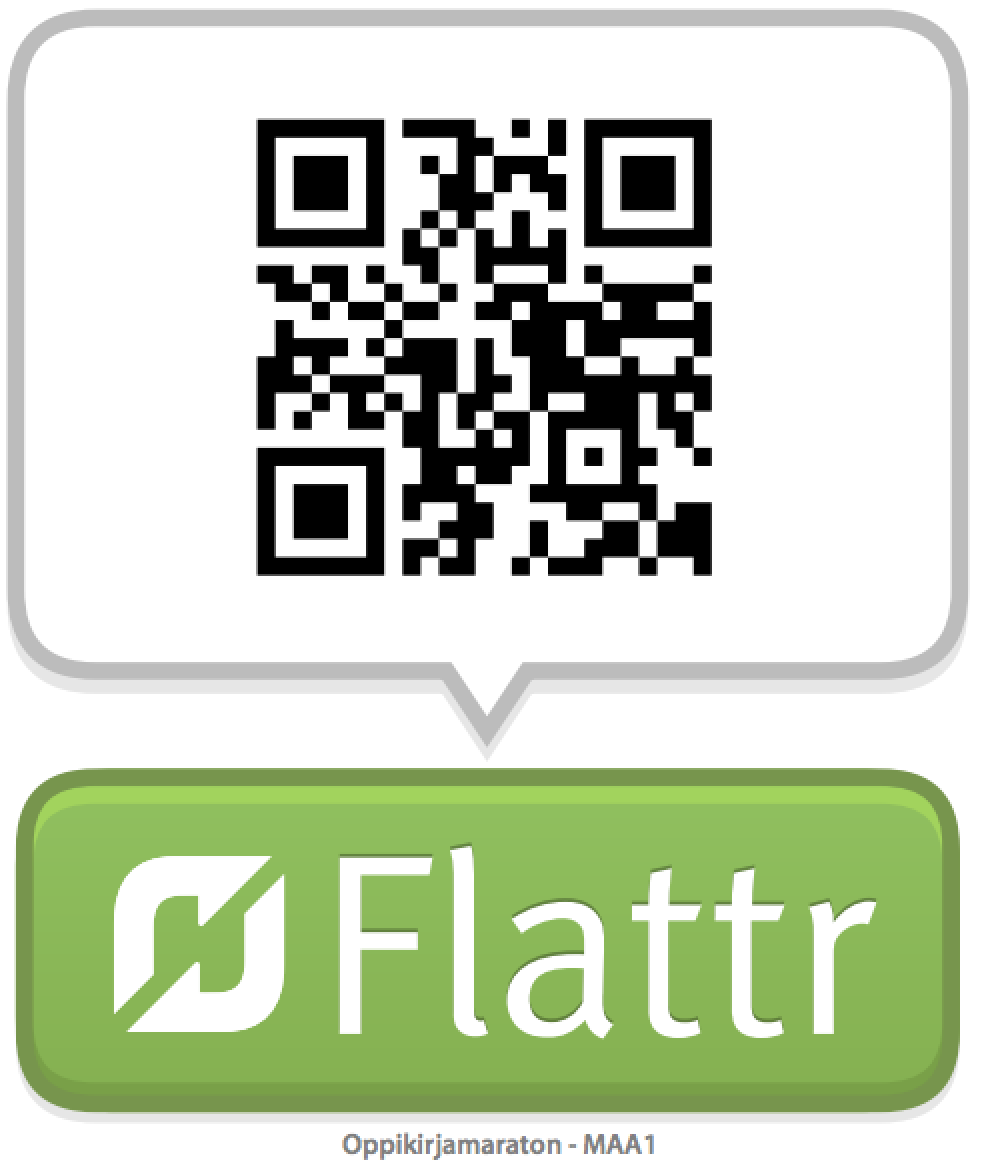
\includegraphics[scale=0.2]{MAA1-Flattr.png} \\
%\url{http://flattr.com/t/914482}
%
%\subsubsection*{Bitcoin}
%
%
\includegraphics[scale=0.2]{Oppikirjamaraton-Bitcoin.png} \\
%bitcoin:148pMeTViRMFBqMVZRnMZ6Hwccq9WTubq1?label=Oppikirjamaraton

\subsubsection*{Lisätietoja kirjasta}

Kirjan virallinen kotisivu: \url{http://avoinoppikirja.fi} \\
Oppikirjamaraton Facebookissa: \url{http://facebook.com/oppikirjamaraton} \\
Avoimet oppimateriaalit ry \& Oppikirjamaraton IRCnetissä: \#avoimetoppimateriaalit
